\documentclass[aspectratio=169]{beamer}
\usetheme{Madrid}
\usecolortheme{beaver}

\usepackage[UTF8,fontset=fandol]{ctex}
\usepackage{amsmath, amssymb}
\usepackage{booktabs}
\usepackage{ragged2e}
\usepackage{array}
\usepackage{tikz}
\usetikzlibrary{positioning, arrows.meta}

\newcolumntype{L}[1]{>{\RaggedRight\arraybackslash}p{#1}}

\title[0514report]{0514report}
\subtitle{}
\date{2026-05-14}

\begin{document}

\begin{frame}
    \titlepage
\end{frame}

% ============================================================
\section{当前结论}
% ============================================================

\begin{frame}[t]{三周汇报主线}
\small
\begin{columns}[T]
\begin{column}{0.31\textwidth}
\textbf{1. Scope 扩散}
\begin{itemize}
    \item LLM 判断 \texttt{scope\_amplitude}
    \item 本地 embedding 相似度矩阵决定扩散方向
    \item Gaussian 权重把负面归因扩散到相似任务
    \item 主要影响其他任务的 \texttt{task\_self\_efficacy}
\end{itemize}
\end{column}

\begin{column}{0.31\textwidth}
\textbf{2. Stream memory}
\begin{itemize}
    \item 复用 AgentSociety 原生 \texttt{status + stream + search}
    \item 写入 raw episode
    \item 在 appraisal / attribution / interview 前检索相关经历
    \item 不新建第二套 memory 系统
\end{itemize}
\end{column}

\begin{column}{0.31\textwidth}
\textbf{3. 行动机制链（贝叶斯方法）}
\begin{itemize}
    \item 降低旧 \texttt{rule\_weights} 对行动选择的直接控制
    \item 接入 \texttt{semantic\_v2} 作为 LLM reference policy
    \item 跑通 Bayesian gated-lite2 的低扰动 action-outcome 学习层
    \item 新增 Huys--Dayan-inspired controllability audit / modulation
\end{itemize}
\end{column}
\end{columns}
\end{frame}

\begin{frame}[t]{主要修改内容}
\small
\begin{columns}[T]
\begin{column}{0.49\textwidth}
\textbf{Scope 扩散}
\begin{itemize}
    \item LLM 只判断 \texttt{scope\_amplitude}
    \item 本地代码用 embedding 算出的 task-family 相似度矩阵
    \item Gaussian 权重决定扩散到哪些相似任务
    \item 扩散扣的是其他任务的 \texttt{task\_self\_efficacy}
\end{itemize}
\end{column}

\begin{column}{0.49\textwidth}
\textbf{Stream memory}
\begin{itemize}
    \item 复用原生 \texttt{status + stream + search}
    \item 写入 raw episode 与检索相关经历
    \item 只服务 appraisal / attribution / interview
    \item 不新建第二套 memory 系统
\end{itemize}
\end{column}
\end{columns}

\vspace{0.2cm}
\end{frame}

% ============================================================
\section{Scope 扩散}
% ============================================================

\begin{frame}[t]{Scope 扩散在系统里的位置}
\small
\centering
\vspace{0.65cm}
\begin{tikzpicture}[
    node distance=0.72cm,
    box/.style={rectangle, rounded corners, draw=black!55, fill=black!4,
        align=center, minimum width=2.6cm, minimum height=0.72cm},
    arrow/.style={-{Latex[length=2mm]}, thick, draw=black!70}
]
\node[box] (event) {负面数字事件};
\node[box, right=of event] (attrib) {event attribution};
\node[box, right=of attrib] (amp) {\texttt{scope\_amplitude}};
\node[box, below=of amp] (gauss) {Gaussian spillover};
\node[box, left=of gauss] (se) {相似任务\\self-efficacy 下降};
\node[box, left=of se] (future) {后续任务\\更易回避/失败};

\draw[arrow] (event) -- (attrib);
\draw[arrow] (attrib) -- (amp);
\draw[arrow] (amp) -- (gauss);
\draw[arrow] (gauss) -- (se);
\draw[arrow] (se) -- (future);
\end{tikzpicture}

\vspace{0.45cm}
\begin{minipage}{0.78\textwidth}
\justifying
LLM 负责主观泛化强度，代码负责把这个强度按任务相似度扩散。
\end{minipage}
\end{frame}

\begin{frame}[t]{Scope 扩散公式与触发条件}
\small
\begin{columns}[T]
\begin{column}{0.52\textwidth}
\textbf{本地 Gaussian 公式}
\[
d(i,j)=1-S_{ij}
\]
\[
w_{ij}=\exp\left(-\frac{d(i,j)^2}{2\sigma^2}\right),\quad
\hat{w}_{ij}=\frac{w_{ij}}{\sum_{k\neq i}w_{ik}}
\]
\[
A_t=\beta\cdot U_t\cdot a_t,\quad
\Delta SE_{j,t}^{spill}=-A_t\hat{w}_{ij}
\]
\end{column}

\begin{column}{0.44\textwidth}
\textbf{默认参数}
\begin{itemize}
    \item \texttt{BETA=1.2}
    \item \texttt{THRESHOLD=0.15}
    \item \texttt{SIGMA=0.45}
\end{itemize}

\vspace{0.1cm}
\textbf{触发条件}
\begin{itemize}
    \item 负面 outcome
    \item attribution 状态为 \texttt{ok}
    \item \texttt{scope\_amplitude} 达到阈值
\end{itemize}
\end{column}
\end{columns}

\end{frame}

\begin{frame}[t]{embedding计算任务相似度矩阵}
\scriptsize
\centering
\renewcommand{\arraystretch}{1.06}
\begin{tabular}{@{}lcccccc@{}}
\toprule
 & Nav & Login & Search & Form & Service & Payment \\
\midrule
Nav & 1.000 & 0.635 & 0.692 & 0.620 & 0.746 & 0.603 \\
Login & 0.635 & 1.000 & 0.517 & 0.717 & 0.626 & 0.598 \\
Search & 0.692 & 0.517 & 1.000 & 0.621 & 0.711 & 0.693 \\
Form & 0.620 & 0.717 & 0.621 & 1.000 & 0.695 & 0.615 \\
Service & 0.746 & 0.626 & 0.711 & 0.695 & 1.000 & 0.643 \\
Payment & 0.603 & 0.598 & 0.693 & 0.615 & 0.643 & 1.000 \\
\bottomrule
\end{tabular}

\vspace{0.14cm}
\begin{minipage}{0.94\textwidth}
\scriptsize
\justifying
\textbf{用于 embedding 的任务描述示例（入口导航与服务定位）：}
用户刚进入一个数字服务时，需要从首页、菜单、搜索框、分类标签或个人中心中判断应该点击哪里，找到目标功能入口。这个任务的核心困难不是输入信息，而是理解页面结构、识别图标含义、在多个入口之间做选择，并在跳转后确认自己没有走错路径。常见失败包括找不到目标服务、点进错误页面、返回后迷路、页面层级太深。
\end{minipage}

\vfill
{\raggedright\tiny
备注：相似度矩阵用智谱 \texttt{embedding-3} 对任务描述做向量编码，再计算余弦相似度。\par}
\vspace*{-0.12cm}
\end{frame}

% ============================================================
\section{Memory 设计}
% ============================================================

\begin{frame}[t]{复用原生 AgentSociety memory}
\small
\begin{columns}[T]
\begin{column}{0.48\textwidth}
\textbf{原生结构}
\begin{itemize}
    \item \texttt{KVMemory}: key-value 状态
    \item \texttt{StreamMemory}: 时间顺序经历流
    \item \texttt{VectorStore}: 语义检索
    \item \texttt{Memory}: 暴露 \texttt{status} 与 \texttt{stream}
\end{itemize}
\end{column}

\begin{column}{0.48\textwidth}
\textbf{我们复用了}
\begin{itemize}
    \item 写入：\texttt{memory.stream.add}
    \item 检索：\texttt{memory.stream.search}
    \item topic 分类语义
    \item 原生返回文本格式
\end{itemize}
\end{column}
\end{columns}

\vspace{0.18cm}
\scriptsize
\textbf{写入的 description 示例：}\\
\texttt{[digital\_task\_episode][family=payment\_risk\_confirmation]}\\
\texttt{[outcome=failure\_after\_attempt][strategy=try\_self]}\\
\texttt{[help=false][uncontrollability=0.82]}\\
我这次自己尝试支付结算，但还是失败了。页面反复报错，这让我感觉这件事不太受自己控制。\\
\vspace{0.08cm}
\textbf{检索返回时的原生外层格式：}\\
\texttt{- [digital\_task\_episode]: description [day: ..., time: ..., location: ...]}
\end{frame}

\begin{frame}[t]{Stream Memory 接入流程}
\scriptsize
\vspace{1.05cm}
\renewcommand{\arraystretch}{1.18}
\begin{tabular}{@{}L{0.18\linewidth}L{0.30\linewidth}L{0.44\linewidth}@{}}
\toprule
环节 & 做什么 & 接入点 \\
\midrule
写入 & 记录经历流 & 任务、求助、恢复等经历都写进 \texttt{stream}，保持时间顺序和 topic 分类 \\
检索 & 回忆相关经历 & 在 appraisal / attribution / interview 前按 topic 和 query 取回相关内容 \\
审计 & 记录使用痕迹 & retrieval 会带上 condition、status、hash、count 等审计信息 \\
\bottomrule
\end{tabular}
\end{frame}

\begin{frame}[t]{旧 rule 现在在哪里}
\small
\begin{columns}[T]
\begin{column}{0.48\textwidth}
\textbf{旧版本更像}
\begin{itemize}
    \item 根据 helplessness、support、difficulty 等计算 \texttt{rule\_weights}
    \item \texttt{rule\_weights} 更直接参与 action weight
    \item 行动倾向更容易被解释成 hand-coded strategy
\end{itemize}
\end{column}

\begin{column}{0.48\textwidth}
\textbf{当前 \texttt{semantic\_v2}}
\begin{itemize}
    \item \texttt{pi\_ref = weak neutral prior + bounded LLM weights}
    \item \texttt{rule\_weights} 保留为 context / audit / fallback
    \item 不再直接混入 \texttt{semantic\_v2} 的 \texttt{pi\_ref}
\end{itemize}
\end{column}
\end{columns}

\vspace{0.32cm}
\begin{minipage}{0.91\textwidth}
\justifying
需要诚实区分：我们降低的是 rule 对当前 action selection 的直接控制；心理状态更新仍然是显式 post-outcome state-transition，用于保证轨迹稳定、可审计、可复现。
\end{minipage}
\end{frame}

\begin{frame}[t]{当前主流程}
\centering
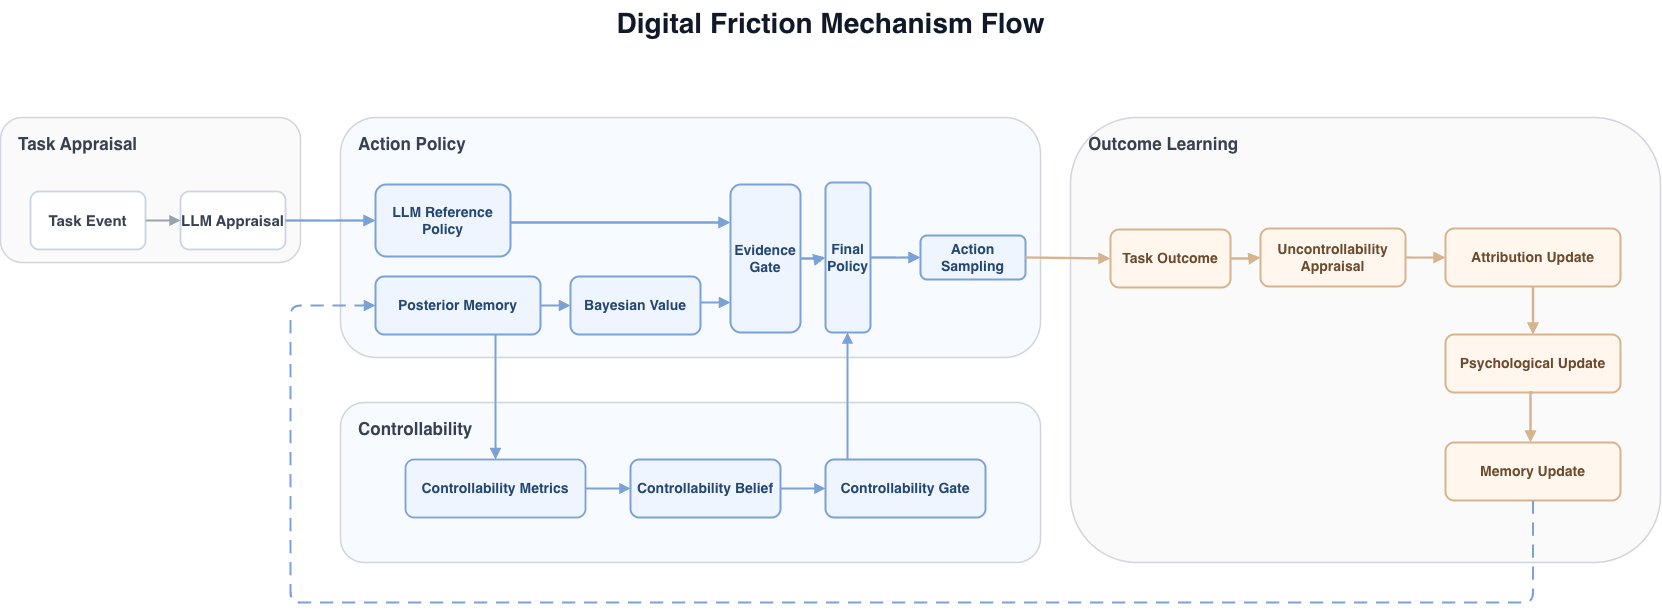
\includegraphics[width=\textwidth,height=0.82\textheight,keepaspectratio]{digital_friction_bayesian_gated_lite2_aaai_architecture_0514_mechanismnames.drawio.png}
\end{frame}

\begin{frame}[t]{当前流程怎么读}
\small
\begin{columns}[T]
\begin{column}{0.31\textwidth}
\textbf{左侧：任务理解}
\begin{itemize}
    \item Task Event 先进入 LLM Appraisal
    \item LLM 结合任务、心理状态和记忆判断难度、风险、控制感
    \item 输出作为后续 reference policy 的语义基础
\end{itemize}
\end{column}

\begin{column}{0.31\textwidth}
\textbf{中间：行动策略}
\begin{itemize}
    \item LLM Reference Policy 给出 \texttt{pi\_ref}
    \item Bayesian posterior 计算 \texttt{Q\_bayes} / \texttt{pi\_bayes}
    \item Huys--Dayan-lite 给出 controllability modulation
    \item Evidence gate 形成最终行动分布
\end{itemize}
\end{column}

\begin{column}{0.31\textwidth}
\textbf{右侧：结果学习}
\begin{itemize}
    \item action 后生成 Task Outcome
    \item 再更新 uncontrollability、attribution、psychology
    \item outcome 后才写回 memory
    \item 写回信息只影响未来 event
\end{itemize}
\end{column}
\end{columns}
\end{frame}

% ============================================================
\section{行动机制链：semantic + Bayesian + controllability}
% ============================================================

\begin{frame}[t]{semantic\_v2：LLM Reference Policy}
\small
\begin{columns}[T]
\begin{column}{0.48\textwidth}
\textbf{旧问题}
\begin{itemize}
    \item 旧 \texttt{rule\_weights} 更直接参与行动权重
    \item 容易被解释成 hand-coded strategy
\end{itemize}
\end{column}

\begin{column}{0.48\textwidth}
\textbf{当前做法}
\vspace{0.12cm}
\begin{minipage}{0.94\textwidth}
\justifying
心理状态更新仍然是显式 post-outcome state-transition，用于保证轨迹稳定、可审计、可复现。
\end{minipage}
\end{column}
\end{columns}

\end{frame}

\begin{frame}[t]{Bayesian gated-lite2：action-outcome posterior}
\small
\begin{columns}[T]
\begin{column}{0.50\textwidth}
\textbf{posterior policy layer}
\begin{itemize}
    \item Bayesian posterior 估计 \texttt{P(outcome | family, action)}
    \item 用 \texttt{Q\_bayes} 与 softmax 得到 \texttt{pi\_bayes}
    \item confidence / entropy gate 控制是否介入
    \item \texttt{max\_delta} 限制每次行为扰动
\end{itemize}
\end{column}

\begin{column}{0.46\textwidth}
\textbf{接入方式}
\begin{itemize}
    \item 先读取 \texttt{pi\_ref}
    \item 再计算 \texttt{pi\_bayes}
    \item gate 打开时才小幅移动 policy
    \item outcome 后写回 posterior memory
\end{itemize}
\end{column}
\end{columns}
\end{frame}

\begin{frame}[t]{Bayesian 相关文献讲了什么}
\small
\begin{columns}[T]
\begin{column}{0.49\textwidth}
\textbf{Balleine \& Dickinson (1998)}
\begin{itemize}
    \item 目标导向行动不只是 stimulus-response habit
    \item 个体会学习 action 与 outcome 的 contingency
    \item outcome 是否有价值会改变行动倾向
    \item 所以行动需要同时考虑“我做什么会发生什么”和“这个结果值不值得”
\end{itemize}
\end{column}

\begin{column}{0.49\textwidth}
\textbf{Huys \& Dayan (2009)}
\begin{itemize}
    \item behavioral control 不是单个 action 的成功率
    \item controllability 取决于 action 是否能可靠改变 outcome distribution
    \item 关键概念包括 outcome entropy、achievable outcomes、controllably achievable value
    \item 还强调不可控经验可能泛化到新环境
\end{itemize}
\end{column}
\end{columns}

\vspace{0.20cm}
\begin{minipage}{0.92\textwidth}
\justifying
我们的设计只取这两层思想：先用 action-outcome posterior 表示“做什么会导致什么”，再从 posterior 派生轻量 controllability diagnostic，判断任务是否看起来可控。
\end{minipage}
\end{frame}

\begin{frame}[t]{Huys--Dayan-inspired controllability}
\small
\begin{columns}[T]
\begin{column}{0.50\textwidth}
\textbf{要补的理论层}
\begin{itemize}
    \item Phase4 学的是 \texttt{action -> outcome}
    \item Huys--Dayan-lite 关心的是行动是否能可靠地产生有价值结果
    \item 从 posterior 中派生 \texttt{C\_family}
    \item 再形成平滑的 \texttt{C\_global} trace
\end{itemize}
\end{column}

\begin{column}{0.46\textwidth}
\textbf{和原论文的相似点和取舍}
\begin{itemize}
    \item 都关心 action 是否改变 outcome
    \item 都强调 outcome reliability / entropy
    \item 都关心有价值结果是否可达
    \item 暂不做 full RL，避免引入 planning 与 transition model
\end{itemize}
\end{column}
\end{columns}
\end{frame}

\begin{frame}[t]{C\_family 的三个组成部分}
\small
\renewcommand{\arraystretch}{1.16}
\begin{tabular}{@{}L{0.25\linewidth}L{0.35\linewidth}L{0.32\linewidth}@{}}
\toprule
指标 & 通俗含义 & 注意事项 \\
\midrule
\texttt{entropy\_control} & 某个 action 的 outcome 是否稳定、可预测 & 低熵不等于结果好，总是失败也可能低熵 \\
\texttt{action\_contrast} & 不同 action 是否真的带来不同 outcome 分布 & 用 coarse outcome bins，避免 subtype 标签夸大差异 \\
\texttt{chi\_lite} & 有价值结果是否能被 action 达到 & 重点看 success / controllable recovery，而不是任意稳定结果 \\
\bottomrule
\end{tabular}

\vspace{0.35cm}
\[
C_{family}=0.25\cdot entropy + 0.25\cdot contrast + 0.50\cdot \chi_{lite}
\]

\end{frame}

\begin{frame}[t]{Outcome 分箱：避免把失败误算成好结果}
\small
\centering
\renewcommand{\arraystretch}{1.13}
\begin{tabular}{@{}L{0.28\linewidth}L{0.58\linewidth}@{}}
\toprule
coarse bin & outcome subtype \\
\midrule
success & \texttt{success\_self}, \texttt{success\_with\_help} \\
controllable failure & \texttt{failure\_after\_attempt\_low\_uncontrollability} \\
uncontrollable failure & \texttt{failure\_after\_attempt\_mid\_uncontrollability}, \texttt{failure\_after\_attempt\_high\_uncontrollability}, \texttt{failure\_even\_with\_help} \\
dropout & \texttt{abandon\_midway} \\
no task evidence & \texttt{no\_attempt} \\
unknown & \texttt{neutral\_unknown} \\
\bottomrule
\end{tabular}

\vspace{0.35cm}
\begin{minipage}{0.86\textwidth}
\justifying
\texttt{failure\_after\_attempt\_low\_uncontrollability} 不应放进 success。它更像“失败了，但仍有可学习、可调整的控制信号”。
\end{minipage}
\end{frame}

\begin{frame}[t]{Huys--Dayan-inspired controllability 调节}
\small
\begin{columns}[T]
\begin{column}{0.50\textwidth}
\textbf{Low C flatten-only}
\[
\gamma=\delta_{max}\cdot conf\cdot\frac{T_{low}-C}{T_{low}}
\]
\[
\pi'=(1-\gamma)\pi_{base}+\gamma\pi_{uniform}
\]
\begin{itemize}
    \item 不直接推 \texttt{seek\_help}
    \item 不直接推 \texttt{avoid}
    \item 含义：低可控性削弱 action preference contrast
\end{itemize}
\end{column}

\begin{column}{0.46\textwidth}
\textbf{High C reduce-avoid}
\[
\delta=\delta_{max}\cdot conf\cdot\frac{C-T_{high}}{1-T_{high}}
\]
\begin{itemize}
    \item 从 \texttt{avoid} 移出小幅概率
    \item 给 Phase4 \texttt{pi\_final} 或 \texttt{Q\_bayes} 支持的最佳 non-avoid action
    \item 不默认转向 \texttt{attempt\_self}
\end{itemize}
\end{column}
\end{columns}
\end{frame}

\begin{frame}[t]{Phase5B 0514 smoke run}
\small
\centering
\renewcommand{\arraystretch}{1.16}
\begin{tabular}{@{}L{0.43\linewidth}L{0.43\linewidth}@{}}
\toprule
指标 & 0514 smoke 结果 / 含义 \\
\midrule
设置 & 1 seed, 4 worlds, 10 days, Huys gate = 0.20, \texttt{confidence\_k=4} \\
policy payload coverage & 1.0，Bayesian policy audit 正常写入 \\
Huys payload coverage & 1.0，controllability audit 正常写入 \\
post-outcome leakage & 未发现，当前 action 不读取当前 outcome \\
Bayesian intervention rate & 约 6.53\%，仍是保守调节 \\
Huys intervention rate & 约 6.34\%，降低 gate 后开始触发 \\
Huys mean TVD & 约 0.000023，说明行为扰动极小 \\
\bottomrule
\end{tabular}

\vspace{0.32cm}
\begin{minipage}{0.88\textwidth}
\justifying
0513 Phase4 pilot 已先验证 Bayesian gated-lite2 的 coverage、no leakage 与低扰动接入；0514 进一步把 Huys--Dayan-lite 分支接到 final policy。结论：该分支已经能接入并触发，但当前 single-stage smoke run 中行为效应很弱，更适合证明工程安全与可审计性，不能直接作为最终机制因果证据。
\end{minipage}
\end{frame}

\begin{frame}[t]{后续计划}
\small
\begin{minipage}{0.74\textwidth}
\textbf{多 agent 想法}
\begin{itemize}
    \item 第一阶段只做 HelperAgent / FamilyHelperAgent
    \item 只在 \texttt{seek\_help} 时触发
    \item 输出结构化 \texttt{support\_response}
    \item 暂不做大规模社交网络或自由聊天
\end{itemize}
\end{minipage}

\end{frame}

\end{document}
